% options:
% thesis=B bachelor's thesis
% thesis=M master's thesis
% czech thesis in Czech language
% slovak thesis in Slovak language
% english thesis in English language
% hidelinks remove colour boxes around hyperlinks

\documentclass[thesis=B,english]{FITthesis}[2012/06/26]
\usepackage[utf8]{inputenc} % LaTeX source encoded as UTF-8

\usepackage{cite}
\usepackage{graphicx} %graphics files inclusion
\usepackage{hyperref}
\usepackage{csquotes}
\usepackage{listings,xcolor}
\usepackage{float}

% \usepackage{amsmath} %advanced maths
% \usepackage{amssymb} %additional math symbols

\usepackage{dirtree} %directory tree visualisation
% % list of acronyms
% \usepackage[acronym,nonumberlist,toc,numberedsection=autolabel]{glossaries}
% \iflanguage{czech}{\renewcommand*{\acronymname}{Seznam pou{\v z}it{\' y}ch zkratek}}{}
% \makeglossaries
\setlength{\textfloatsep}{0.1cm}

\newcommand{\tg}{\mathop{\mathrm{tg}}} %cesky tangens
\newcommand{\cotg}{\mathop{\mathrm{cotg}}} %cesky cotangens

\department{Department of Software Engineering}
\title{Open data of Prešov}
\authorGN{Juraj}
\authorFN{Šprlák}
\authorWithDegrees{Juraj Šprlák}
\supervisor{Mgr. Jan Starý, Ph.D.}
\acknowledgements{I would like to thank to my}
\abstractCS{V~několika větách shrňte obsah a přínos této práce v~češtině. Po přečtení abstraktu by se čtenář měl mít čtenář dost informací pro rozhodnutí, zda chce Vaši práci číst.}
\abstractEN{Sem doplňte ekvivalent abstraktu Vaší práce v~angličtině.}
\placeForDeclarationOfAuthenticity{Prague}
\declarationOfAuthenticityOption{4} %volba Prohlášení (číslo 1-6)
\keywordsCS{Otvorené dáta, štátna správa, webová aplikácia, mesto Prešov, Java}
\keywordsEN{Open data, state service, web application, Prešov, Java}

\begin{document}

% \newacronym{CVUT}{{\v C}VUT}{{\v C}esk{\' e} vysok{\' e} u{\v c}en{\' i} technick{\' e} v Praze}
% \newacronym{FIT}{FIT}{Fakulta informa{\v c}n{\' i}ch technologi{\' i}}

\begin{introduction}
	Impact of information is great nowadays. Internet helps people in everyday's life to get the information about almost everything almost immediately and to make decisions.
	Neither the public affairs did not escape this phenomenon. The society is getting more and more interested in transparency of state government. The idea of Open data was created to satisfy this demand. They can provide the evidence that public money is being well spent and proclaimed policies are being implemented. Publishing state economy data, public procurements, tax declarations, even fortune of politicians or private companies and other data on public web servers is a common practice in many developed countries.
	\par Thanks mainly to the European Union and other international institutions, but also enthusiasts and engaged citizens, more and more projects targetting electronisation, systematisation and publishing the data are being started also in Slovakia. The idea to publish in machine-readable form all that is not secret or personal data it still young, though, and often meets unwillingness or incompetence of the public institutions. As a result, quite often the data published by Slovak state and municipality governments, proclaimed to be open, are useless due to their non-machine-readable formats, incompleteness or lack of interconnectivity.
		Despite these problems, some progress has been made in this area in recent years and the number of datasets published by state institutions grows every day. Thanks to that there is a growing potential for software developers to create applications for manipulating, inteconnecting, analysing and presenting these data and thus turning them into useful information. This is one of the goals of this thesis.
	\section*{Open data of Prešov}
	Looking at the datasets published on the official website of Slovak government - \href{https://data.gov.sk}{data.gov.sk} one easily discovers, that the most active of all the cities and towns in Slovakia in publishing the data is Prešov. Not only by number of published datasets, but also by quality of the data this city in eastern Slovakia shares the most from its governing with its citizens. These data include all past contracts, invoices, orders and grants of the municipality. That is why these data were chosen for the purpose of this bachelor thesis.
	\section*{Thesis Goals}
	The main goal of this thesis is to analyse, interconnect and present the economic open data of Prešov municipality to demonstrate their value and usefulness for the citizens. Focus is on interconnecting them by logical ties not only to each other, but also to other published open data in Slovakia, e.g. Slovak Business Register. This requires analyses of all published open data in Slovakia. The final product of the thesis is a web application to present the analysed and interconnected data. A final goal is to present the application to the Prešov city officials and try to convince them to publish and run it on their web servers, so it can serve the public. Other goals of this work are to explain the general concept of open data, the attributes, that such data need to have, describe international institutions focusing on the open data with influence on Slovakia, discuss the best practises and world leaders in opening the government data and introduce the most influential Slovak state and non-state open data projects and initiatives.

\end{introduction}

\chapter{Open data}
	This chapter is devoted to the problematics of open data. It provides knowledge about what the open data are, what are their main attributes, explains these attributes and informs about open data situation in Europe and some of the important organisations concerned with open data and open government.
	\section{Definition}
	Open data are data that are accessible, can be used, re-used and redistributed by anyone for free (or no more than reproduction cost), subject only, at most, to the requirement to attribute and share-alike\footnote{Share-alike is a copyright term, describing works that require copies or adaptations of the work to be released under the same or similar licence as the original.}. For the sake of interoperability (i.e. ability of diverse systems and organisations to work together) the exact definition of open data is crucial. \cite{opendatahandbook} 
	\section{Requirements}
	Requirements that open data need to meet are the following:\cite{opendefinition}
	\renewcommand\labelitemii{}
	\begin{itemize}
	 	\item \textbf{Open license}
			\begin{itemize}
				\item The work must be available under an open license. Any additional terms accompanying the work (such as a terms of use, or patents held by the licensor) must not contradict the terms of the license.
		\end{itemize}
  		\item \textbf{Access}
  			\begin{itemize}
  				\item The work shall be available as a whole and at no more than a reasonable one-time reproduction cost, preferably downloadable via the Internet without charge. Any additional information necessary for license compliance (such as names of contributors required for compliance with attribution requirements) must also accompany the work.
  			\end{itemize}
  			\item \textbf{Open Format}
  			\begin{itemize}
  				\item The work must be provided in a convenient and modifiable form such that there are no unnecessary technological obstacles to the performance of the licensed rights. Specifically, data should be machine-readable, available in bulk\footnote{Data is available in bulk if the whole dataset can be downloaded easily. It is considered non-bulk if the citizens are limited to getting parts of the dataset through an online interface.}, and provided in an open format or, at the very least, can be processed with at least one free/libre/open-source software tool.
  			\end{itemize}
	\end{itemize}

To understand the requirements properly, next part is devoted to explaining the most important points mentioned above.
	\subsection{Open licenses}
	\label{licenses}
	Open data need to be available under an open license. A licence tells anyone the conditions, under which they can access, use and share the data. Unless the data have a licence, data may be ‘publicly available’, but users do not have permission to access, use and share it under copyright or database laws. A license is open if it:
	\begin{itemize}
		\item allows free use and redistribution (including sale) of the licensed work.
		\item allows creation of derivatives of the work and their distribution under the same terms
		\item does not impose any fee arrangement as part of its conditions
		\item does not discriminate against any person or group
	\end{itemize} 
	The next part looks at some of the most common open licenses. 
	\subsubsection{Creative commons}
	Creative Commons (CC) is a non-profit organisation devoted to the idea of making the creative works available for others to legally build upon and share. Among other activities it provides free copyright licenses to make a simple and standardized way to give the public permission to share and use creative work on conditions of choice. \cite{creativecommons}
	\paragraph{CC Attributon-ShareAlike}
	lets people remix, tweak, and build upon the licensed work even for commercial purposes, as long as they credit the owner and license their new creations under the identical terms. This is the license used by Wikipedia, and is recommended for materials that would benefit from incorporating content from Wikipedia and similarly licensed projects.
	\paragraph{CC0}
	is the "no copyright reserved" option - it means giving up all copyright rights that the owner of the work holds and dedicating those rights to the public domain under copyright law, to the extent allowed by law.
	\paragraph{CC Attribution}
	allows re-distribution and re-use of a licensed work on the condition that the creator is appropriately credited.
	\subsubsection{GNU Free Documentation License}
	The GNU Free Documentation License is a copyleft license - which means that derivative works must be made available under the same or a similar license. The creators of the license recommend that it is used “principally for works whose purpose is instruction or reference".
	\subsubsection{Open government licenses}
	\label{opengovernmentlicense}
	Some governments have chosen to develop their own licenses for the data they publish. The good examples are France\footnote{Available at \url{https://www.etalab.gouv.fr/licence-ouverte-open-licence}} and Britain\footnote{Available at \url{http://www.nationalarchives.gov.uk/doc/open-government-licence/version/3/}}.
	\subsection{Data file formats}
	\label{fileformats}
	 File format is the digital base in which the information is stored. For the open data to be easily usable, the correct file format is crucial. Choosing the format depends mainly on the character of the data (e.g. structured data for statistics, geodata for geographic data displayed in map, etc.). The formats in which information is published can either be “open” or “closed”. If a file format is “closed”, this may be either because the file format is proprietary and the specification is not publicly available, or because the file format is proprietary and even though the specification has been made public, re-use is limited. Releasing information in a closed file format can cause significant obstacles to reusing the information encoded in it, forcing those who wish to use the information to buy the necessary software. Open format is a file format with a freely available published specification which places no restrictions upon its use. The preference from the open government data perspective therefore is that information be released in open file formats which are machine-readable. Following are the data formats that are most-widely used for data publishing by government institutions.\cite{opendatahandbookfileformats}
	 
	 	\subsubsection*{JSON}
	 	JSON is a simple file format that is very easy for any programming language to read. Its simplicity means that it is generally easier for computers to process than others, such as XML.
	 	\subsubsection*{XML}
	 	XML is a widely used format for data exchange because it gives good opportunities to keep the structure in the data and the way files are built on, and allows developers to write parts of the documentation together with the data without interfering with the reading of them.
	 	\subsubsection*{RDF} 	
		RDF makes it possible to represent data in a form that makes it easier to combine data from multiple sources. RDF data can be stored in XML and JSON, among other serialisations. RDF encourages the use of URLs as identifiers, which provide a convenient way to directly interconnect existing open data on the Web. RDF is still not widespread, but it has been a trend among Open Government initiatives, including the British and Spanish Government Linked Open Data projects.
		\subsubsection{CSV, XLS/XLSX}
		CSV, or Comma Separated Values can be a very useful format because it is compact and thus suitable to transfer large sets of data with the same structure. It is particularly important for the comma-separated formats that documentation of the individual fields are accurate.
Furthermore it is essential that the structure of the file is respected, as a single omission of a field may disturb the reading of all remaining data in the file without any real opportunity to rectify it, because it cannot be determined how the remaining data should be interpreted.
Many authorities have information left in the spreadsheet, for example Microsoft Excel. In this case, it is stored in XLS format, which is closed (and thus not suitable for open data), or XLSX format, which is partially open. This data can often be used immediately with the correct descriptions of what the different columns mean.
		\subsubsection{Text formats, PDF, TXT}
		Classic documents in formats like Word (closed format), ODF, OOXML, or PDF may be sufficient to show certain kinds of data - for example, relatively stable mailing lists or equivalent. It may be cheap to exhibit in, as often it is the format the data is born in. The format gives no support to keep the structure consistent, which often means that it is difficult to enter data by automated means. Use of templates as the basis of documents is important to make it possible to pull information out of documents.
Plain text documents (.txt) are very easy for computers to read. They generally exclude structural metadata from inside the document however, meaning that developers will need to create a parser that can interpret each document as it appears.
\paragraph{}Most data need further processing (to save the data in the database, connect the data to other sources, etc.). As the data can be too big to manualy process, manipulating with them should be automatable. The best formats to make automatization of the data more convenient are the structured ones like JSON, XML and RDF. On the contrary, images and text formats like PDF are very difficult to process. Spreadsheet formats (XLS/XLSX, CSV) are structured, but their structure is easily corrupted and manipulating data in these formats is usually less convenient.

	\subsection{Data openness levels}
	Tim Berners-Lee, the inventor of the Web and Linked Data initiator, suggested a 5-star deployment scheme for Open Data. This scheme, shown in \ref{fig:5-star} picture, is widely used (e.g. by British government open data) to rate given data based on their attributes like file format, structure, inteconnectivity, etc.


	\section{Open data in the world}
	\textbf{Open data barometer} is a World Wide Web Foundation's global measure of how governments are publishing and using open data for accountability, innovation and social impact.\cite{opendatabarometer} \paragraph{} Barometer ranks governments on:
\begin{itemize}
	\item readiness for open data initiatives
	\item implementation of open data programmes
	\item impact that open data have on business, politics and civil society
\end{itemize}
The ranking made by Open data Barometer in 2016 is the following:
\begin{center}
\begin{tabular}{l}
  \textbf{1.} Great Britain \\
  \textbf{2.} Canada \\
  \textbf{3.} France \\
  \textbf{4.} USA \\
  \textbf{5.} South Korea \\
  \\
  \textbf{29.} Slovakia \\
  \textbf{31.} Czech Republic \\
\end{tabular}
\end{center}
  \subsection{Great Britain's open data}
  Great Britain is the global leader in opening government data. It scored 100/100 in the overal assesment of the prevalence of open data initiatives of Open data barometer.
  There are several reasons why the UK's open data are ranked so well. One of them is its ‘Open Data Readiness’, which is the policy framework for the release of open data. It includes having national guidelines that are applicable to specific sectors, and these guiding principles ensure a smooth release of open data that can benefit anyone that wishes to access it.

Government’s Digital Service Standard provides guidelines on data publishing. A number of regional or city initiatives are integrated into the \linebreak\href{https://data.gov.uk}{data.gov.uk} portal, too, such as Open Manchester, Leeds Data Mill, Birmingham Open Data, Bristol City Council Open Data, to mention just a few.

The UK Government Licensing Framework provides a policy and legal framework for licensing the use and re-use of public sector information across the public sector. It sets out best practices, standardises the licensing principles for government information, mandates the Open Government Licence (OGL) as the default licence for Crown bodies and recommends OGL for other public sector bodies (see \ref{opengovernmentlicense}).

Following in the UK’s footsteps in open data guidelines would be a good place to start for other countries hoping to improve in this area.\cite{UKopendatagov}

One of the interesting applications of UK's open data is the \textbf{LMI For All} project. It is an online data portal, developed by the UK Commission for Employment and Skills, which brings together existing national sources of high quality labour market information (LMI) that can inform and help people make right choices about their careers. The online portal includes LMI that can help answering the questions people ask when thinking about their careers, like how much people earn or what type of persons do what kind of jobs, etc. It includes information from the Annual Survey of Hours and Earnings, the Labour Force Survey, the Employer Skills Survey and Working Futures. All of its data are made freely available  via an Application Programming Interface (API) for use in websites and applications.

Other interesting applications built using UK's open data can be seen at \href{https://data.gov.uk/apps}{data.gov.uk/apps}. These include Car Insurance Comparison Application, All GB Railway Stations, Inheritance Tax Calculator UK and more.


	\subsection{Open Government Partnership}
	Open Government Parthership (OGP) is the international governments initiative, which was launched in 2011 by 8 founding governments (Brasil, Indonesia, Mexico, Norway, Philippines, South Africa, United Kingdom and United States). The focus of the initiative is the improvement of government by promoting transparency, efectiveness and responsibility, harnessing new technologies and setting up institutions, which help citizens to participate in governing. To become a member of OGP, participating countries must commit to uphold the principles of open and transparent government by endorsing the \href{https://www.opengovpartnership.org/open-government-declaration}{Open Government Declaration}. In total there are over 70 OGP participating countries and 15 subnational governments and together they have made over 2,500 commitments to make their governments more open and accountable. \cite{opengovernmentpartnership}
	
	\subsection{European Union initiatives}
\textbf{European Union Open Data Portal}, set up in 2012, is the open data portal of the European Union containing datasets that are collected and published by the European Institutions and other EU bodies. It provides a standardized catalogue of EU open data and a list of applications and web tools reusing these data. \cite{EUopendataportal}
\hspace{10000px}
The \textbf{European Data Portal} is an initiative of the European Commission, and is part of the Digital Single Market. It was created to gather Public Sector Information of the 28 European Member States and the four EFTA (Norway, Iceland, Switzerland and Liechtenstein) countries. Information regarding the provision of data and the benefits of re-using data is also included. Going beyond the harvesting of metadata, the strategic objective of the European Data Portal is to improve accessibility and increase the value of Open Data. Within the Portal, sections are dedicated to searching datasets, providing data, using data, training and library. It also contains ratings of open data of every involved country. \cite{eudataportal}

\chapter{Open data in Slovakia}
	Slovakia ranked 29th in the above mentioned Open data barometer for 2016. It moved 7 places up the ranking since 2015. European Data portal publishes factsheets, which summarize readinnes, challenges and shortcommings of open data in each member country. According to 2017 factsheet dedicated to Slovakia, the main possitives of Slovak open data are: presence of action plan of Open Government for 2017-2019; presence of national guidelines on data publication; data licensing 100\% free of charge and big amount of regional data initiatives. On the contrary, the main negatives/barriers are: less then 25\% of the data uploaded automatically; lack of integrated regional portals; passive approach of Open Data holders, mainly by municipalities and lack of promotion of prescribed technical standards. \cite{eudataportalfactsheet}
	\section{Political support}
	A lot of positive steps were made towards open government in Slovakia during the short government of Iveta Radičová (2010-2012). Most notable ones were making publishing of contracts on the internet mandatory (see \ref{crz}) and introduction of electronical auction for public procurements. On 20th September 2011, the Government of the Slovak Republic joined the Open Government Partnership and in 2012 approved the first  action plan for the Open Government Initiative for years 2012-2013, which created an open data portal. In June 2016, a new  office -- Deputy Prime Minister's office for Investments and Informatization was set up, with one of the main tasks being creation and implementation of uniform state policy in the field of informatization of the society. In March 2017, \href{https://www.opengovpartnership.org/sites/default/files/Slovakia_NAP_2017-2019_EN.pdf}{Open Government Partnership National Action Plan} for years 2017-2019 was adopted by the Slovak government. This plan addresses open data (by formulating new commitments on publicly available APIs and open source software), open education, public policy making and open justice.
	\section{Slovak open data portal - data.gov.sk}
	Official government open data portal - data.gov.sk was launched in 2013 as part of the Open Government Initiative, which aims to improve governance through increasing transparency, efficiency and accountability. Declared goals of the portal are publishing data and metadata (data describing data like column descriptors, etc.) in machine-readable form using open standards and licenses. The website allows users to search datasets by organisation that published them, license, file formats and tags. It also supports a full-text search by name and description of a dataset and even by its location on the map.
	Following are some statistics from the portal (March 2018):
	\begin{itemize}
		\item 4399 unique visitors on average per month
		\item 30\% of the visitors foreign 
		\item most datasets available in CSV format
		\item  99\% of the datasets machine-readable
		\item 66 organisations publishing data
		\item 1425 datasets available
	\end{itemize}
	The most active organisations by number of published datasets:
	\begin{center}
	\label{toporganisations}
        \begin{tabular}{  p{0.65\linewidth} | c }
        \textbf{organisation} & \textbf{Number of datasets} \\ \hline
        Slovak Statistical Office & 625 \\
        Public Procurement Office & 64 \\
        The city of Prešov & 58 \\
        Ministry of Interior of the Slovak republic & 57 \\
        Central Agricultural Control and Testing Institute & 43 \\
        \end{tabular}
    \end{center}
    \vspace{20px}
    The most commonly used file formats (many datasets are published in more than one file format):
    \begin{center}
        \begin{tabular}{  p{0.65\linewidth} | c }
        \textbf{File format} & \textbf{Number of datasets} \\ \hline
        CSV & 877 \\
        XML & 336 \\
        HTML & 218 \\
        XLSX & 185 \\
        JSON & 11 \\
        \end{tabular}
    \end{center}
    \vspace{20px}
    The most commonly used licenses (see \ref{licenses}):
    \begin{center}
        \begin{tabular}{  p{0.65\linewidth} | c }
        \textbf{License} & \textbf{Number of datasets} \\ \hline
        Creative Commons Attribution Share-Alike & 737 \\
        Creative Commons CCZero & 87 \\
        Creative Commons Attribution & 24 \\
        Other non-commercial & 14 \\
        GNU Free documentation license & 7 \\
        \end{tabular}
    \end{center}
    \vspace{20px}
    The most common tags:
    \begin{center}
        \begin{tabular}{  p{0.65\linewidth} | c }
        \textbf{Tag} & \textbf{Number of datasets} \\ \hline
        Statistics & 607 \\
        Key tables & 190 \\
        Elections & 177 \\
        Key Indicators & 98 \\
        Parliament & 63 \\
        \end{tabular}
    \end{center}
    \section{Other state projects}
    Beside the above-described official Slovak open data portal, several other big state-run projects are present. The most important ones are Central Register of Contracts and Business register.
    \subsection{Central Register of Contracts}
    \label{crz}
    	Started on 1st January 2011, Central Register of Contracts (available at \href{https://www.crz.gov.sk}{crz.gov.sk}) is a website containing contracts (with their appendices and  attachments) concluded by so-called obliged entities - Government Office, ministries, central government authorities, public bodies and their subordinate organisations (contributors, budgetary organisations, etc.) since the beginning of 2011. As of March 2018, the database contains 1 578 659 contracts. All contracts concluded prior to 2011 are available at older address \href{http://www.zmluvy.gov.sk}{zmluvy.gov.sk}. The operator of both websites is the Government Office of the Slovak Republic. 
    	
    	The register has proven to be successful. The procurement costs of public orders fell by almost one third in the very first year of the register’s operation due to reduced financial mismanagement. Iveta Radičová, former Slovak Prime Minister during whose government the project was started, described its success in these words:
\begin{displayquote}“Following the first year of the register’s operation, savings in public finances amounted to an average of 30 percent of costs. There were also some areas – for example, the transport sector – where the savings reached 50 percent. The Office of the Government alone saved EUR 3.5 million in the first year of the register’s operation. The publication of a contract also prevented an overpriced purchase of flowers for EUR 10 000 at the Ministry of Education.”\cite{joinupcrz}
\end{displayquote}
    \section{Business register}
    \label{businessregister}
     The Business Register (available at \href{http://www.orsr.sk}{orsr.sk}) is a public registry that contains particular information specified by the law about individual entrepreneurs, companies and other legal entities. The registry is owned and maintained by the Ministry of Justice of Slovakia. It can be searched by business name, identification number, registered seat, registration number or name of a person. The register provides information from January 2001 onwards.

	\section{Non-state initiatives}
	\label{non-state-initiatives}
	In addition to the official projects of Slovak republic and municipalities, there are several civic associations, non-profit organisations and private companies dedicated to state open data. Some of them are trying to improve the quality and usefullness of the available data, others interconnect them with other sources and present them in an attractive form. Most often their main goal is to bring more transparency to public spending and state government. Next section looks at the most important ones.
	\subsection{Slovensko.digital}
	\label{slovensko.digital}
	\href{https://slovensko.digital}{Slovensko.digital} is a civic association aimed at improving the quality of state digital services in Slovakia. 
	Their goals are sumarized on their website:
	\begin{displayquote}
		"We want the digital services of the state to be simple, meaningful and have a normal price. We need to increase the transparency and efficiency of spending of public resources as well as the participation of the professional public in the electronisation of public administration."
	\end{displayquote}
	In accordance with these goals, slovensko.digital set up the \href{https://platforma.slovensko.digital}{platform} for all IT specialists, who want to join the discussion about state IT projects. This civic association's members also developed a methodology that focuses on more than 50 criteria of project success and use it to systematically rate state IT projects and alert the public to the risky ones in one of their project called \href{https://redflags.slovensko.digital/}{Red Flags}. Thanks to this, slovensko.digital was able to stop a couple of senseless state projects, saving Slovak citizens hundreds of millions of euros. They've also started several projects as part of \href{https://ekosystem.slovensko.digital/}{ekosystem.slovensko.digital}, some of which provide APIs to public data sources (otherwise only accessible on websites) like Register of legal entities, Central register of contracts, Public procurement journal, Business journal, Registry of financial statements and more. 
	\subsection{Finstat}
	\label{finstat}
	\href{https://finstat.sk/}{Finstat} was started in 2013 as a web portal, which helps people to freely assess financial health of Slovak companies. It connects data from various data sources: ministries, state insurance companies, Business register, Statistical office, Slovak Chamber of executors, Trade Journal, Register of enterpreneurs, Register of financial statements, Register of bankrupts, Czech statistical office and many more and by their processing and analysing provides complex information about Slovak companies, individual sectors and groups of enterpreneurs. The portal also helps media and non-profit organisations to analyse companies and investigating corruption cases by development of analyses and making the data of the portal accessible for them. A lot of its features are for free and some features, like API access and datasets in CSV are parts of payed packages.
	\subsection{Uvostat}
	\label{uvostat}
	\href{https://www.uvostat.sk/about}{Uvostat} is a project that processes public procurements data, analyses and presents them in the form of statistics and interactive graphs. The statistics include most valuable procurements, most procurements by company or by contracts concluded. The website enables searching in the list of suppliers and even fulltext search in names and contents of the procurements. It also provides notificator for tenders for new positions in state offices, which can be used by people looking for jobs to inform them that a new position which fits their profesion and location is being opened. The interesting fact about the project is that it has been developed by only two people.
	\subsection{Otvorené zmluvy (Open contracts)}
	\href{http://www.otvorenezmluvy.sk/o-projekte}{Otvorené zmluvy} is an investigative project of Slovak anti-corruption initiative Aliance Fair-play and Transparency International, which helps citizens to read, search and assess contracts concluded by state and state institutions, which are being published by law since 2011. It offers automated analyses and offers general public to join discussions (crowdsourcing), trying to draw attention to suspicious contracts.	
	\subsection{Datanest}
	\href{http://datanest.fair-play.sk/}{Datanest} was also created by Aliance Fair-play as a source of information about management of Slovak public money as part of their anti-corruption initiatives. It serves mainly journalists, analytics, watchdog organisations, but also engaged citizens. It contains data generated by state since 1990, which in some cases can't yet be obtained in electronic form elsewhere.
	\subsection{foaf.sk}
	\href{http://foaf.sk}{Foaf.sk} draws information about Slovak companies from publicly available Business register, Business journal, Registry of financial statements, database of Social insurance agency debtors, Financial Administration, and other databases. The website uses graph algorithms to look for and display deeper connections between people and companies in Slovakia, which enables users to quickly search for and display relations between companies and enterpreneurs. The name FOAF comes from the English acronym \textit{Friend Of A Friend} and refers to the phenomenon of the \href{http://www.scholarpedia.org/article/Small-world_network}{small world networks}.

	
\chapter{Analyses of the Prešov open data}
\label{presovopendata}
	The city of Prešov is the only municipality in Slovakia, which is in the top 10 organisations by number of published datasets on data.gov.sk (see \ref{toporganisations}). Prešov is also the only municipality in Slovakia, that provides open geodata. At ITAPA\footnote{ITAPA events (Information Technologies and Public Administration) are the most important and well–known IT events in Slovakia since 2002.\cite{itapa}} 2017 awards, the city's webgis geodata\footnote{data about geographic locations, that can be displayed in a map} \href{http://webgis.presov.sk/}{project} was awarded 3rd place. Mariana Hurná, Prešov's main IT coordinator was awarded as Best IT specialist of Slovak municipalities in years 2008, 2009 and 2012. The city maintains \href{http://egov.presov.sk}{egov.presov.sk} information system  portal to enable its citizens access to useful information about city data. Published here are data about street names, members of municipal government, members of municipal police, camera systems locations, demographic structure of citizens of the city, drawing of the municipality budget, register of petitions, tax debtors and more. Prešov is by all means a very good example of municipality that works towards greater  transparency by processing the data it collects from the citizens. Unlike most other Slovak municipalities, its employees don't only do the necessary minimum to comply with the law, but also do the additional work to provide useful data applications and progress to its citizens.
	
	\section{Prešov contracts, grants, invoices and orders}
	\label{presovdataattributes}
	Slovak municipalities are obliged to publish data about orders, contracts and invoices of institutions like City Office, Municipal Police, Registry office and all budgetary organisations of which they are founders. This is mandatory by law 211/2000\footnote{Available at \url{http://www.zakonypreludi.sk/zz/2000-211}} in Slovak collection of laws. Additionally, Prešov municipality  publishes all applications for grants to comply with its internal binding regulations. Prešov publishes this data on its website \url{egov.presov.sk}, as well as on the national open data portal \url{data.gov.sk}, in various formats (XML, JSON, XLSX, and PDF) under Creative Commons Attribution license (see \ref{licenses}). Next sections look at the data that are used in practical part of these bachelor thesis - contracts, invoices, grants and orders. They provide basic statistics of each of these datasets and describes their attributes. All the statistics were collected from egov.sk on April 8th 2018.
	\subsection{Contracts}
        \begin{tabular}{  p{0.5\linewidth}  l }
        \\
        Total published contracts & 6027 \\
        Oldest contract published on & August 2nd 2011\\
        Latest contract published on & April 6th 2018 \\
        \end{tabular}
        
    \begin{center}
        \begin{tabular}{  p{0.7\linewidth} | p{0.3\linewidth} }
        Attribute & Data type\\ \hline
        id (central number) & Integer \\
        type & String \\
        contracting parties & String \\
        subject & String \\
        total price & Integer \\
        currency & String \\
        date of signature & Date \\
        date of release & Date \\
        name (detailed type) & String \\
        parties' national identifiers & String \\
        parties' addresses & String \\
        notes & String \\
        main/appendix indicator & String \\
        effective date & Date \\
        \end{tabular}
    \end{center}
	\subsection{Invoices}
	\begin{tabular}{  p{0.5\linewidth}  l }
        \\
        Total published invoices & 28511 \\
        Oldest invoice published on & May 26nd 2011\\
        Latest invoice published on & April 6th 2018 \\
        \end{tabular}
        
    \begin{center}
        \begin{tabular}{  p{0.7\linewidth} | p{0.3\linewidth} }
        Attribute & Data type\\ \hline
        id (internal number) & Integer \\
        name of the organisation & String \\
        supplier & String \\
        payment purpose description & String \\
        total price & Integer \\
        currency & String \\
        id of contract & Integer \\
        id of order & Integer \\
        release date & Date \\
        supplier national identifier & String \\
        supplier address & String \\
        payout status & String \\
        office & String \\
        invoice number & Integer \\
        final/deposit indicator & String \\
        status & String \\
        \end{tabular}
    \end{center}
	\subsection{Orders}
	\begin{tabular}{  p{0.5\linewidth}  l }
        \\
        Total published orders & 28511 \\
        Oldest orders published on & May 26nd 2011\\
        Latest orders published on & April 6th 2018 \\
        \end{tabular}
        
    \begin{center}
        \begin{tabular}{  p{0.7\linewidth} | p{0.3\linewidth} }
        Attribute & Data type\\ \hline
        id & Integer \\
        supplier & String \\
        order text & String \\
        total value & Integer \\
        currency & String \\
        creation date & Date \\
        release date & Date \\
        supplier national identifier & Integer \\
        supplier address & String \\
        office & String \\
        name of approver & String \\
        function of approver & String \\
        date of issue & Date \\
        release notes & String \\
        status & String \\
        contract id & Integer \\
        year of contract & Integer \\
        \end{tabular}
    \end{center}	
	\subsection{Grant applications}
	\begin{tabular}{  p{0.5\linewidth}  l }
        \\
        Total published grant applications & 825 \\
        Oldest grant app. published in & 2012\\
        Latest grant app. published in & 2018 \\
        \end{tabular}
        
    \begin{center}
        \begin{tabular}{  p{0.7\linewidth} | p{0.3\linewidth} }
        Attribute & Data type\\ \hline
        year of dotation & Integer \\
        type & String \\
        status & String \\
        event & String \\
        approved amount & Integer \\
        currency & String \\
        applicant & String \\
        applicant's address & Integer \\
        applicant's city & String \\
        applicant's national identifier & Integer \\
        \end{tabular}
    \end{center}	
	
	\chapter{Implementation}
	As mentioned in the previous chapters, the main output of this bachelor thesis is a website built on top of the economic open data of Prešov. This website not only presents these data and enables searching them, but also provides added value by connecting them to the Slovak Business Register data. Next sections look at how this web application works, how it manages and presents the data and what technologies it uses.   It is divided into four sections dedicated to: data retrieval and processing into database; implementation of the web application; section describing it with screenshots from running application and finally, the comparison between this solution and other applications focused on Open data in Slovakia.
	\section{Data management}
	\subsection{Data from Prešov web server}
	As described in chapter \ref{presovopendata}, the main concern of this web application are data about Prešov's contracts, invoices, orders and applications for grants. These data are being updated daily and can be downloaded in various formats, including XML and JSON, which are structured and thus most suitable for parsing and further use (\ref{fileformats}). JSON format is a more modern alternative to XML and is easier and faster to parse, less memory-consuming and more intuitive to read. That's why the data from Prešov's web servers were downloaded in this format for the purpose of this application. To enable fast searching and accessing these data, they need to be stored in a database. \textit{PostgreSQL}\footnote{PostgreSQL is an open source relational database management system developed by a worldwide team of volunteers. It supports transactions, subselects, triggers, views, foreign key referential integrity, and sophisticated locking and runs on multiple platforms.} was chosen as the database management system. To fill the database with the JSON data, a conversion from JSON to SQL is needed. In this case, this conversion is done by a script written in the \textit{Python} programming language. This script takes JSON file as an input along with the parameter indicating what kind of data are being inserted ("i" for invoices, "c" for contracts, etc.), parses the a JSON file, constructs the SQL CREATE statements to create the database table and indexes for the chosen columns, transforms each JSON object into an SQL INSERT statement and outputs these statements. The result is a series of SQL statements which can be stored as an SQL script and used to fill 4 database tables - Contracts, Invoices, Grants and Orders. The process of getting the data from the web server and transforming it to fill the database is described in the diagram \ref{fig:jsonToDb}.

	\subsection{Data provided by slovensko.digital}
	\label{data-slovensko-digital}
	The data retrieved from Prešov's website contain national identifiers (IČO - organisation identification number) of contract parties, grant applicants and supliers (see \ref{presovdataattributes}). With these identifiers, a given legal entity can be searched in Slovak Business Register (see \ref{businessregister}). The problem of getting the data from this register, which does not provide any API was targetted and solved by slovensko.digital by providing a free API to this register as part of their ekosystem.slovensko.digital project (see \ref{slovensko.digital}). Through this API it is possible to retrieve information about a legal entity with given IČO in JSON format. 
	
	\subsubsection{Data retrievable by IČO}
	To be able to use the above-mentioned API to retrieve the full data about a legal entity by its IČO, the user needs to use an intermediary API, which provides consolidated basic data about the legal entity and also serves as a gateway to other services providing more detailed information. To use this premium intermediary API, an \textit{Authorization token} is required, which needs to be included in the API's URL request header. This token is provided by slovensko.digital upon email request, in which one should describe the purpose of the data usage.\footnote{ The complete guideline describing how to use the API and retrieve the authorization token is available here: https://ekosystem.slovensko.digital/premiove-api\#access-token} The result of a successful request contains the national and tax identifiers, name of the subject, address attributes, dates of establishment and termination, registration office attributes, two system columns describing dates of creation and modification of the entry and finally the URLs to APIs providing more detailed information - full data from Business Register and Register of Accounting Entities. Following is the example of JSON data returned by this API for legal entity with IČO 36421928, which is slovensko.digital:
	\lstset{
    string=[s]{"}{"},
    stringstyle=\color{blue},
    comment=[l]{:},
    commentstyle=\color{black},
    extendedchars=true,
    breaklines=true,
    basicstyle=\fontsize{9}{10}\selectfont,
     literate=%
         {á}{{\'a}}1
         {í}{{\'i}}1
         {é}{{\'e}}1
         {ý}{{\'y}}1
         {ú}{{\'u}}1
         {ó}{{\'o}}1
         {ě}{{\v{e}}}1
         {š}{{\v{s}}}1
         {č}{{\v{c}}}1
         {ř}{{\v{r}}}1
         {ž}{{\v{z}}}1
         {ď}{{\v{d}}}1
         {ť}{{\v{t}}}1
         {ň}{{\v{n}}}1                
         {ů}{{\r{u}}}1
         {Á}{{\'A}}1
         {Í}{{\'I}}1
         {É}{{\'E}}1
         {Ý}{{\'Y}}1
         {Ú}{{\'U}}1
         {Ó}{{\'O}}1
         {Ě}{{\v{E}}}1
         {Š}{{\v{S}}}1
         {Č}{{\v{C}}}1
         {Ř}{{\v{R}}}1
         {Ž}{{\v{Z}}}1                 
}
\begin{lstlisting}
{
   "id":1358414,
   "cin":50158635,
   "tin":2120264674,
   "vatin":null,
   "name":"Slovensko.Digital",
   "formatted_address":"Staré Grunty 6207/12, 841 04 Bratislava - mestská časť Karlova Ves",
   "street":"Staré Grunty",
   "reg_number":6207,
   "building_number":"12",
   "postal_code":"841 04",
   "municipality":"Bratislava - mestská časť Karlova Ves",
   "country":"Slovenská republika",
   "created_at":"2016-06-09T12:26:10.521084Z",
   "updated_at":"2017-06-30T02:10:45.967257Z",
   "established_on":"2016-01-29",
   "terminated_on":null,
   "vatin_paragraph":null,
   "registration_office":"MV SR",
   "registration_number":"VVS/1-900/90-48099",
   "formatted_street":"Staré Grunty 6207/12",
   "street_number":"6207/12",
   "rpo_organisations":[
         {
            "id":6562824,
            "url":"https://datahub.ekosystem.slovensko.digital/api/data/rpo/organisations/6562824"
         }
      ],
   "ruz_accounting_entities":[
         {
            "id":1617045,
            "url":"https://datahub.ekosystem.slovensko.digital/api/data/ruz/accounting_entities/1617045"
         }
      ]
}
\end{lstlisting}

\subsubsection{Full Business Register data}
	Using the URL contained in the above-mentioned data under \emph{rpo\_organisations} attribute, one can obtain full data available for the given entity in the Business Register. These include: list of addresses, legal forms, organisation names, alternate names, predecessors, successors, registration numbers and statutories (with name, address and statutory type). Included are also entity's economic data like economic activity types, money deposits put into the organisation (with name of the depositor and the amount), company equities (investment, paid and approved amounts), shares (with identifiers of shareholder and share price) and stakeholders (name, address and type). All of these entries contain dates of effectiveness from and to, which can be used to construct the history of the legal entity.
\subsubsection{Register of Accounting Entities data}
	The URL under \emph{ruz\_accounting\_entities} attribute points to an API which provides access to data collected from Register of Accounting Entities. This API, however, is only in alpha version and thus only provides limited information like the size of an organisation (by number of employees), ownership type, economic activity, municipality and district.
%\begin{center}
%        \begin{tabular}{ l | l | l }
%Attribute name & Description & Type \\ \hline
%id & Identificator & Integer \\ 
%cin & IČO & Long Integer \\ 
%tin & DIČ & Long Integer \\ 
%vatin & IČ DPH & String \\ 
%name & Názov subjektu & String \\
%formatted\_address & Formatted address & String \\
%street & Ulica & String \\ 
%reg\_number & Súpisné číslo & Integer \\ 
%building\_number & Orientačné číslo & String \\ 
%postal\_code & PSČ & String \\ 
%municipality & Obec & String \\ 
%country && Dátum vzniku & date \\ 
%terminated\_on & Dátum zániku & date \\ 
%vatin\_paragraph & DPH podľa paragrafu & String \\ 
%registration\_office & Registrátor & String \\ 
%registration\_number & Registračné číslo & String \\ 
%formatted\_street & Ulica a číslo & String \\ 
%street\_number & Číslo domu & String \\ 
%created\_at & Čas vzniku záznamu & timestamp \\ 
%updated\_at & Čas poslednej zmeny záznamu & timestamp
%        \end{tabular}
%    \end{center} 

	\section{Web application}
	\subsection{Used technologies}
	The web application was implemented using \emph{Java Platform, Enterprise Edition} (Java EE) technology. \emph{Java Servlet Technology} was used together with \emph{JavaServer Pages} (JSP) to generate web pages based on user request. The application was deployed to \emph{WildFly} application server. \emph{Apache Maven} was used for building the application and dependency management, and \emph{Hibernate ORM} for persistance layer.
	\subsubsection{Java EE}
	Java Platform, Enterprise Edition is a collection of Java APIs that software developers can use to write server-side applications. Its architecture provides services that simplify some common challenges faced by developers building web applications like client requests handling or working with a database.
	\subsubsection{Java Servlet Technology and JSP}
	Java Servlet Technology was created as a way to provide dynamic, user-oriented web content. A servlet is a Java class used to respond to various, most often HTTP requests. JavaServer Pages technology is also used to create web content based on user request. Unlike Java servlet, JaveServer page is not a Java class, but a HTML-like document supporting Java scriptlets, which are pieces of Java-code.
	\subsubsection{Hibernate}
	Hibernate ORM (Object-relational mapping) is a free Java tool, which provides a framework for mapping an object-oriented domain model to a relational database. Its primary feature is mapping from Java classes to database tables and Java data types to SQL data types. Hibernate also supports data querying by generating SQL calls, relieving the developer from manual object conversion.
	\subsubsection{WildFly}
	WildFly, formerly known as JBoss, is a free open-source application server implementing Java EE specification. Being implemented in Java, it can run on multiple platforms.
	\subsubsection{Maven}
	Maven is a build automation tool used mostly in Java projects. It addresses two important parts of software development - describing, how software is built and its dependencies. Is is configured by an XML file called POM (Project Object Model). Maven comes with pre-defined targets for performing tasks as code compilation and packaging. It dynamically downloads libraries and plugins from either its own central repository or ones defined in POM file.
	
	\subsection{Architecture}
	The architecture of the web application is a classic Java Servlet/JSP architecture. The HTTP request is handled by the application server, which finds the correct Java servlet. The servlet then uses application Java classes to do the business logic like retrieving and processing the data from the database or through slovensko.digital's API (this includes parsing the JSON data). After doing the necessery operations the servlet forwards the request to the appropriate JSP document, which handles the UI part. This architecture is described in the diagram \ref{fig:webapp}.


	\section{The website}
	This section describes the application from the user's point of view by describing the contents of pages displayed after successfull call of all the main possible requests (show all contracts, grants, invoices, orders, company, order, contract details, statistics and more) and providing screenshots of these pages.
	
	\subsection{Navigation menu}
	Present at the top of every page, this component provides simple navigation between all the main pages of the application. It contains links to the following pages: all contracts, all grants, all orders, all invoices, statistics of these data and finally the "About" page containing basic information about the application and references to the data sources.
	\subsection{All records pages}
The core of the application are four main pages presenting: all contracts, all grants, all orders and all invoices of the Prešov city. Each of them uses the same layout: top menu toolbar for navigation, data filter, basic statistics (count of records and their total value) and a table containing the data of a given record. The table is paginated - each table page contains 100 records and links to the first, last, previous and next page. If a table contains a name of a company or an enterpreneur (whether it is contract party, grant applicant, or supplier), this name is a link navigating to the detail page of the given company or enterpreneur (presenting the data from the Business register).
	\subsubsection{All Contracts}
	This page providing data of all Prešov's contracts serves as the home page for this application. It presents all contracts from the database. The contracts table contains columns showing the name of the contractor (company or enterpreneur), with which the city of Prešov concluded the contract, subject of the contract (max. first 100 letters), date of signature, contract price and link to the contract detail page. The page filter enables users to filter contracts by the name of the party, subject of the contract and signature date (fields from and to) (see picture \ref{fig:webapp-contracts}).


\subsubsection{Contract detail}
	This page provides complete information of the given contract from the database, including those fields that are not displayed on the all contracts page (see picture \ref{fig:webapp-contract-detail}).


\subsubsection{All Grants}
	This page provides data of all Prešov's orders. The data table contains columns showing the name of the company or enterpreneur, which applied for given grant, related event description (maximum first 100 letters), year of grant and approved money amount. This page's filter enables users to filter grants by the name of the grant applicant and grant event (see picture \ref{fig:webapp-grants}).


\subsubsection{All Orders}
	This page provides data of all Prešov's orders. The data table contains columns showing the name of the  supplier (company or enterpreneur), text of the order (maximum first 100 letters), its value, status, issue date and a link to the order detail page. The data filter enables filtering by the name of the supplier, grant text and issue date (see picture \ref{fig:webapp-orders}).


\subsubsection{Order detail}
	This page provides complete information of the given order from the database, including those fields that are not displayed on the all contracts page (see picture \ref{fig:webapp-order-detail}).


\subsubsection{All Invoices}
	This page provides data of all Prešov's invoices. The data table contains columns showing the name of the  supplier (company or enterpreneur), payment description (maximum first 100 letters), its value, payment status, invoice completeness status, release date and a link to the detail page of related contract or order. The data filter enables filtering by the name of the supplier, payment description and release date (see picture \ref{fig:webapp-invoices}).


\subsection{Legal entity detail}
	The detail page for a legal entity displays the data provided by slovensko.digital from Slovak Business Register (see section \ref{data-slovensko-digital}). A user can navigate to this page by clicking on the name of the company from any webpage containing such link (like all contracts, grants, contract detail, etc.). On the top of this page a basic information about given entity is displayed, with data like IČO, current address, founding date, legal form, ownership type, number of employees, SK NACE classification \footnote{NACE (Nomenclature of Economic Activities) is the European statistical classification of economic activities. NACE groups organisations according to their business activities. \cite{nace}}, place and number of registration and an URL to finstat.sk (see {\ref{finstat} section) page, which provides even more detailed information about it. Right under this basic info section, this page provides the tables with all the Prešov's contracts, grants and orders, that the given entity is involved with. Under these tables, the rest of the available data from the business register follows: tables of economic activities, legal statuses (former and current), statutory bodies, stakeholders,  predecessors and sucessors (if any), equity capital, deposits, former names and addresses, alternate names, authorizations to act on behalf of the entity and past legal forms (if any) (see pictures \ref{fig:webapp-partydetail1}, \ref{fig:webapp-partydetail2}).


\subsubsection{Statistics page}
	The statistics page presents some calculated statistics based on the data presented on the other pages. It is divided into several tabs containing tables, each with top 100 records by specific criteria. It provides: top companies by the total value of paid invoices, top companies by number of paid invoices, top invoices by paid amount, top grants by approved grant amount, top contracts by price, top orders by value. For a better idea, see the \ref{fig:webapp-topcompanies} and \ref{fig:webapp-topinvoices} pictures.

\subsection{Record not found}
	Page like this is displayed, when the contract, order or person with given identifier (contained in the url of the request) was not found in the database. (see picture \ref{fig:webapp-contract-notfound}).
	
	\section{Comparison and possibility of improvements}
	This section focuses on a comparison between the web application created as part of this thesis and other applications presenting Open data in Slovakia. It also disusses possible future enhancements, that could make the application more informative and useful for the users.
	\subsection{Comparison of the solution with other projects}
	There are several interesting projects focusing on open data in Slovakia. Some of them are described in  the section \ref{non-state-initiatives}. Some present similar data, like this application, but all of them are, naturally, more elaborate. One of them is the uvostat (see \ref{uvostat} section) project, which focuses on public procurements and also provides similar statistics (top 100 contracts by value, top 100 companies by the number of finished procurements, etc.). The project is more advanced, though, while it also presents the data in a form of visually appealing interactive graphs and also supports more advanced search. Some similarities can be found with the finstat project (see \ref{finstat} section) in presenting the legal entity details. Finstat also takes data from the Business register, but adds information from other sources (that is why a link to this website is included in the party detail page of this application). It has much a more elaborate layout and presents some data in colorful graphs. 
	\subsection{Possible improvements}
	There are many aspects, which could be improved in this application. One big improvement, that would increase the application's performance and enable more advanced statistics would be not to download the data about a legal entity through the API on each request, but instead store them in the database. This would require a separate program, which would go through all the database records (contracts, invoices, orders and grants), download, parse and store the data about each contractor, supplier, money reciever or grant applicant in the database. This would, for example, allow searching the natural persons with relationships with the companies receiving money from the city budget and make it easier to detect suspicious connections. Other important enhancement would be to include the PDF documents for each contract, order or grant application. This would, however, require a cooperation with the city (granting access to these data), or some complicated algorithm to retrieve these documents from the city's website (the documents are available there, but are not exportable, but instead downloaded upon request for each record). Also, the website only contains contracts, grants and invoices related to the Prešov city itself and not to the subordinate organizations (kindergardens, primary and art schools, senior facilities, etc.). These records are also made available at the website, but are not part of the Open catalogue and thus are difficult to download (they are only exportable from the table view, which doesn't allow downloading more then 10 000 records). In this case, too, a cooperation with the city would be needed to make them provide direct access to these data. A data export would also be a nice feature to have. A lot of improvements could also be done on the UI part of the application, e.g. more advanced layout for the legal entity detail page.
\begin{conclusion}
	%sem napište závěr Vaší práce
\end{conclusion}

\chapter{Figures}
\begin{figure}[H]
  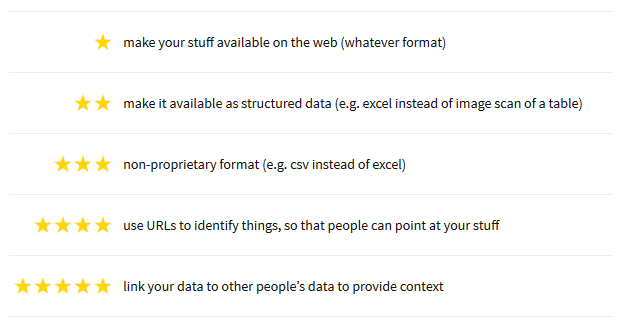
\includegraphics[width=\linewidth]{pictures/5starRating.png}
  \caption{5-star data opennes rating scheme. \cite{5stardata}}
  \label{fig:5-star}
\end{figure}

\begin{figure}[H]
	\centering
	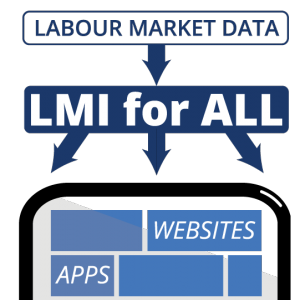
\includegraphics[scale=0.5]{pictures/LMIForAll.png}
  	\caption{LMI for all data providing scheme. \cite{lmiforall}}
  	\label{fig:LMI for all}
\end{figure}

\begin{figure}[H]
  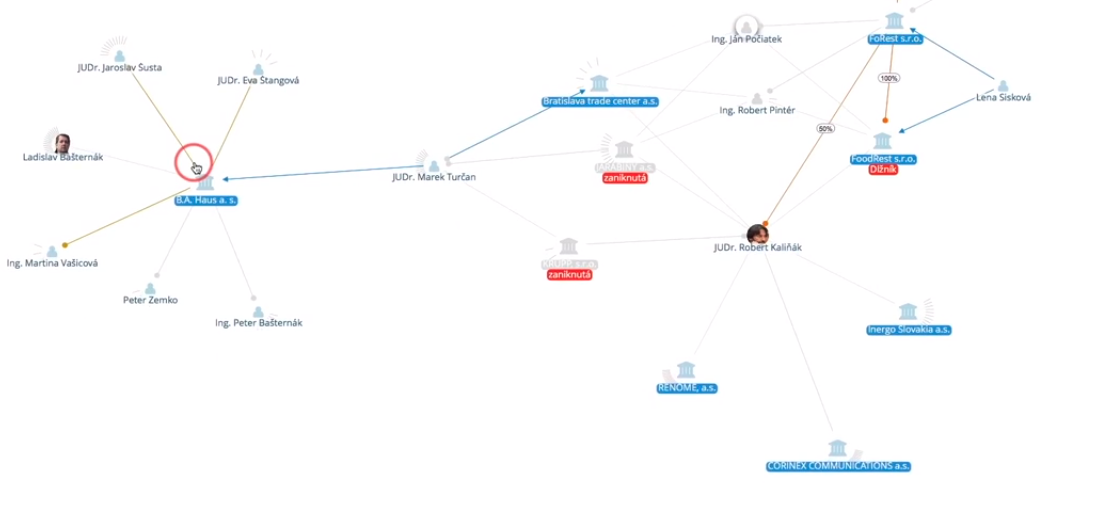
\includegraphics[width=\linewidth]{pictures/foafskgraph.png}
  \caption{Graph created using visualization tool at foaf.sk.}
  \label{fig:foafGraph}
\end{figure}

\begin{figure}[H]
  \begin{center}
  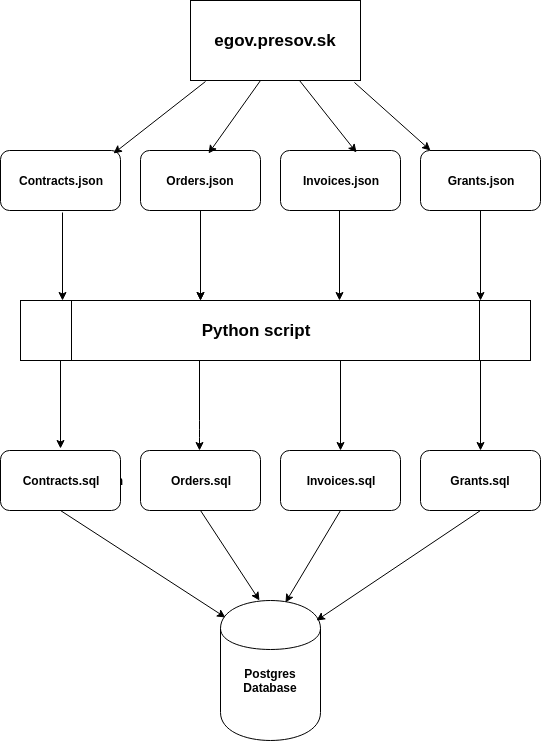
\includegraphics[scale=0.6]{pictures/jsonToDb.png}
  \caption{Diagram describing retrieving the data from egov.presov.sk and transforming it to initialize database.}
  \label{fig:jsonToDb}
  \end{center}
\end{figure}

\begin{figure}[H]
  \begin{center}
  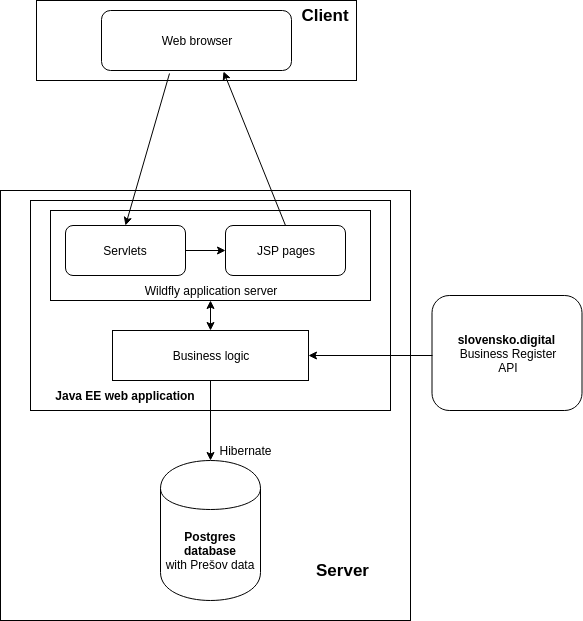
\includegraphics[scale=0.65]{pictures/webappDiagram.png}
  \caption{Diagram describing web application structure.}
    \label{fig:webapp}
  \end{center}
\end{figure}

\begin{figure}[H]
  \begin{center}
  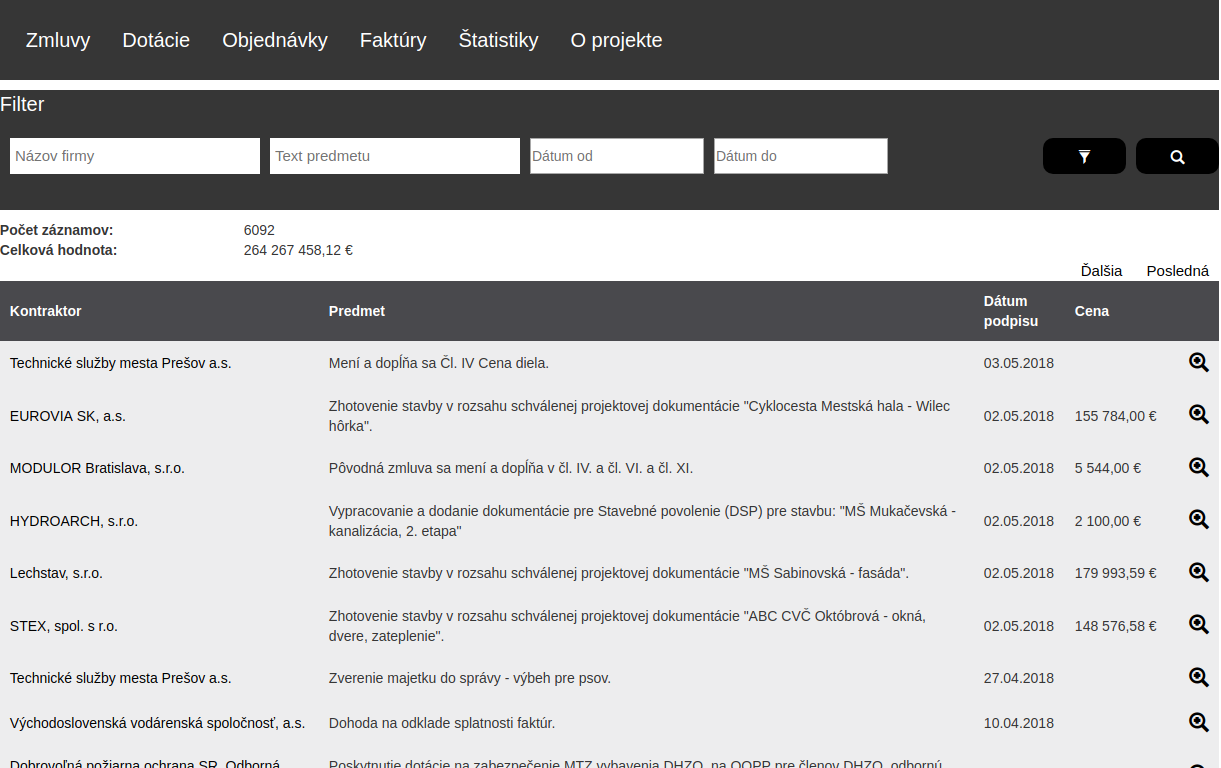
\includegraphics[scale=0.30]{pictures/contracts.png}
  \caption{Picture showing the way the web application presents contracts.}
    \label{fig:webapp-contracts}
  \end{center}
\end{figure}

\begin{figure}[H]
  \begin{center}
  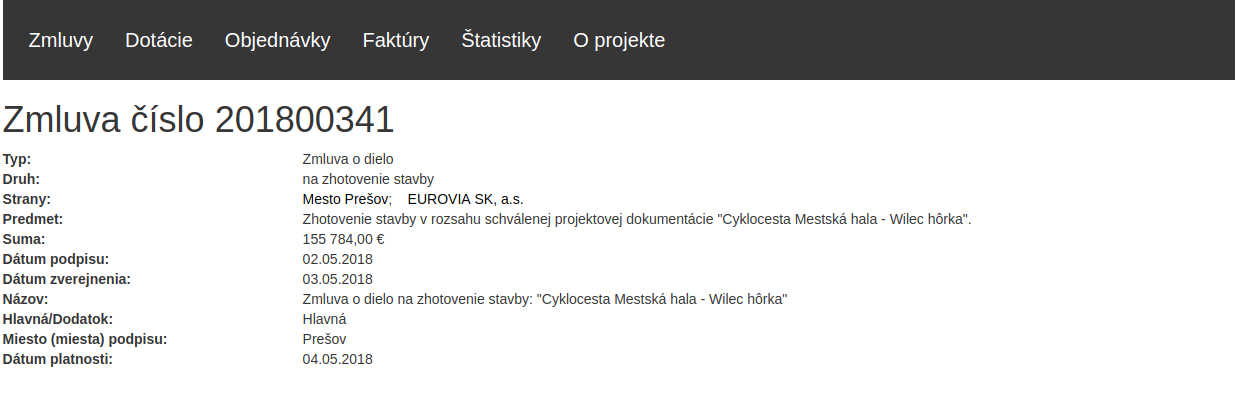
\includegraphics[scale=0.30]{pictures/contractDetail.png}
  \caption{Picture showing the way the web application presents particular contract.}
    \label{fig:webapp-contract-detail}
  \end{center}
\end{figure}

\begin{figure}[H]
  \begin{center}
  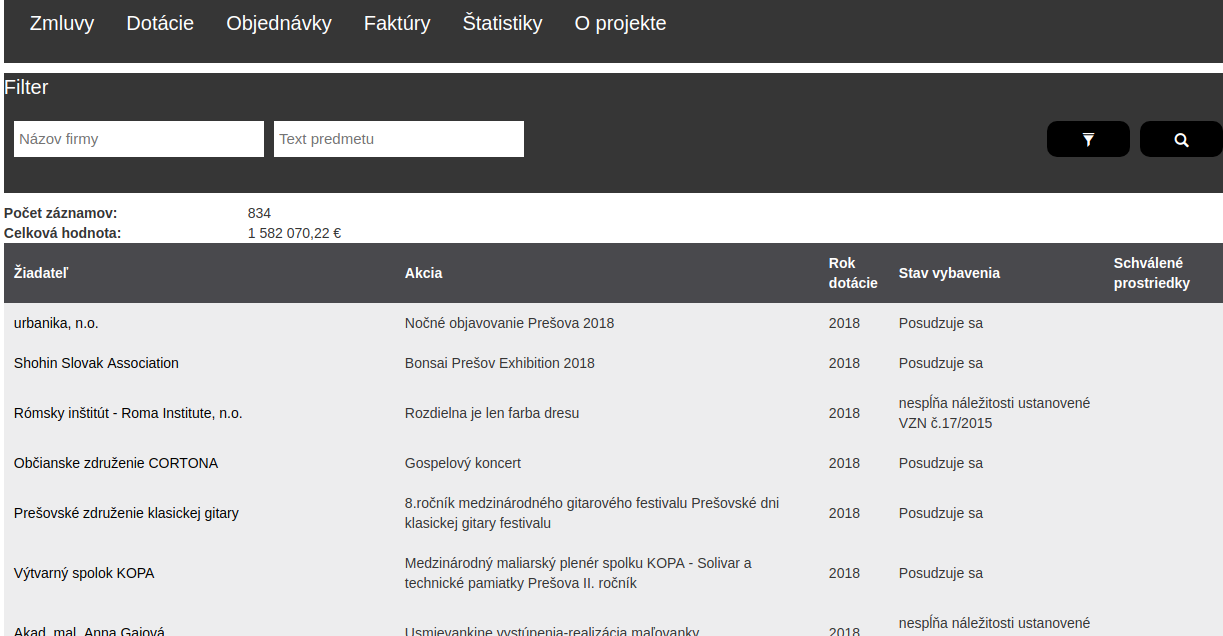
\includegraphics[scale=0.30]{pictures/grants.png}
  \caption{Picture showing the way the web application presents grants.}
    \label{fig:webapp-grants}
  \end{center}
\end{figure}

\begin{figure}[H]
  \begin{center}
  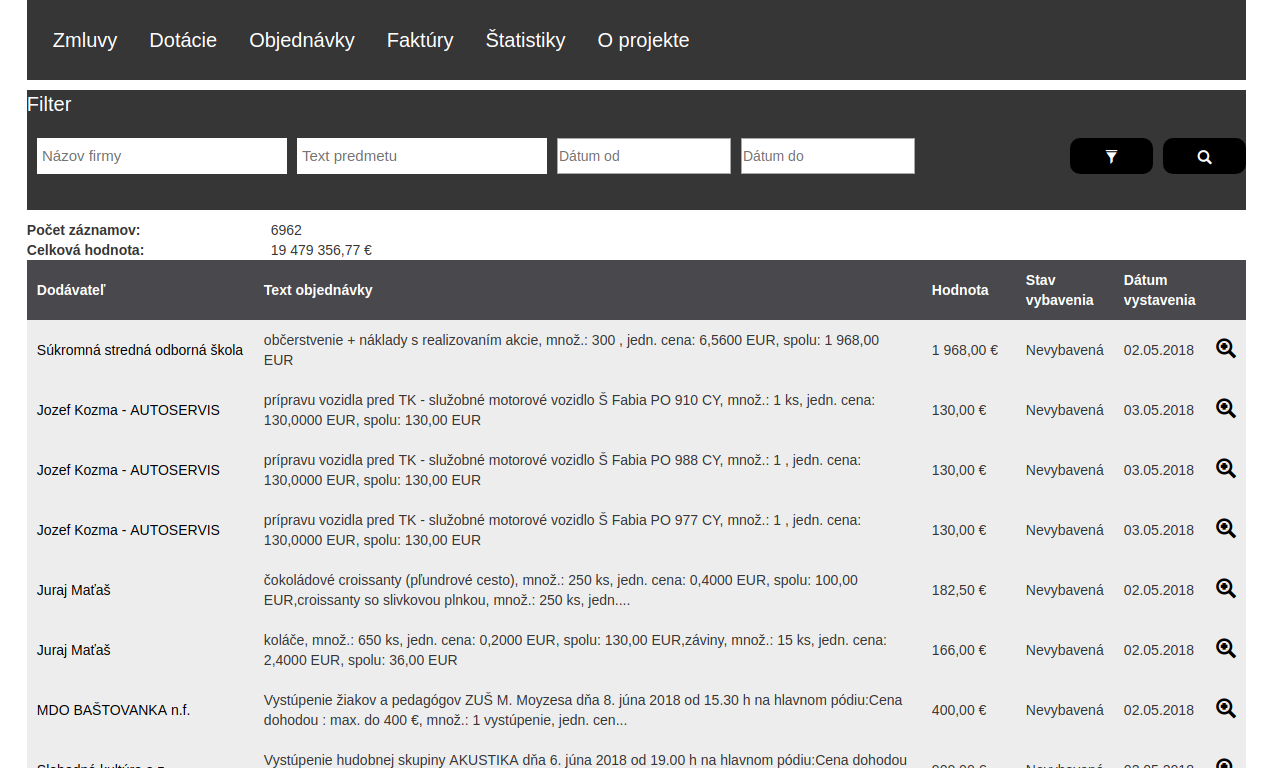
\includegraphics[scale=0.30]{pictures/orders.png}
  \caption{Picture showing the way the web application presents orders.}
    \label{fig:webapp-orders}
  \end{center}
\end{figure}

\begin{figure}[H]
  \begin{center}
  
\includegraphics[scale=0.30]{pictures/orderDetail.png}
  \caption{Picture showing the way the web application presents particular order.}
    \label{fig:webapp-order-detail}
  \end{center}
\end{figure}

\begin{figure}[H]
  \begin{center}
  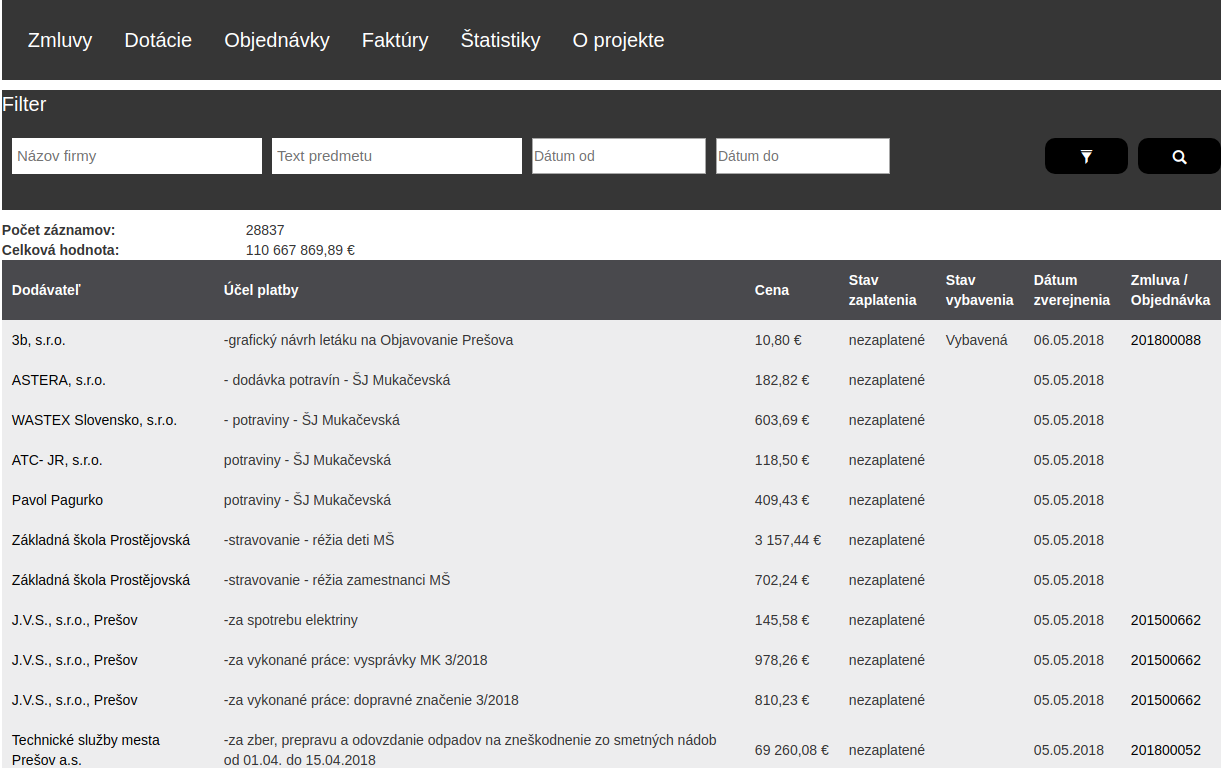
\includegraphics[scale=0.30]{pictures/invoices.png}
  \caption{Picture showing the way the web application presents invoices.}
    \label{fig:webapp-invoices}
  \end{center}
\end{figure}

\begin{figure}[H]
  \begin{center}
  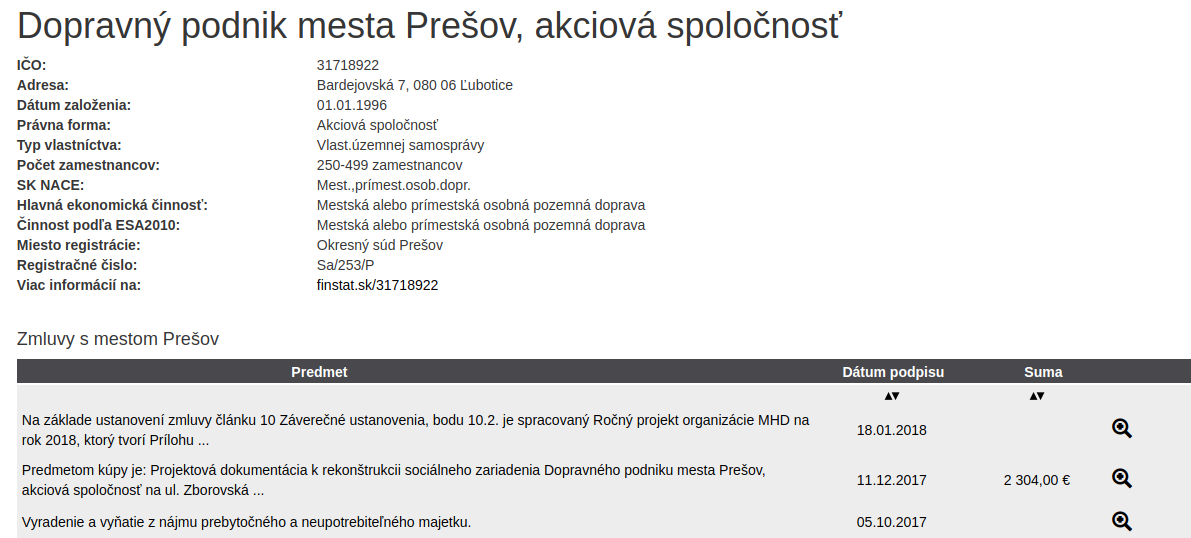
\includegraphics[scale=0.30]{pictures/partyDetail1.png}
  \caption{Basic information of the legal entity and Prešov's contracts it's involved with.}
    \label{fig:webapp-partydetail1}
  \end{center}
\end{figure}
\begin{figure}[H]
  \begin{center}
  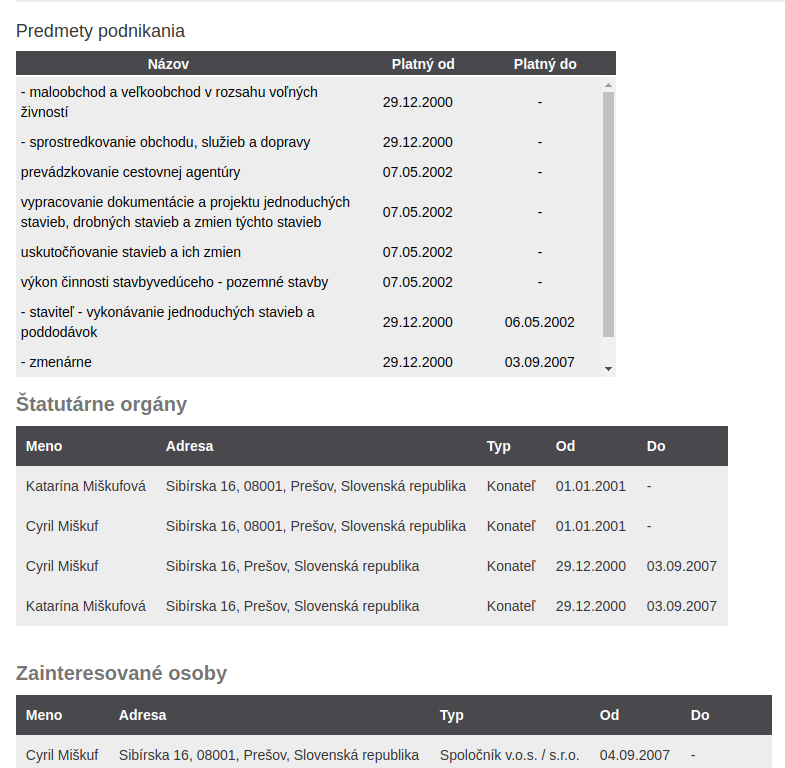
\includegraphics[scale=0.30]{pictures/partyDetail2.png}
  \caption{Economic activities, statutory bodies and stakeholders example.}
    \label{fig:webapp-partydetail2}
  \end{center}
\end{figure}

\begin{figure}[H]
  \begin{center}
  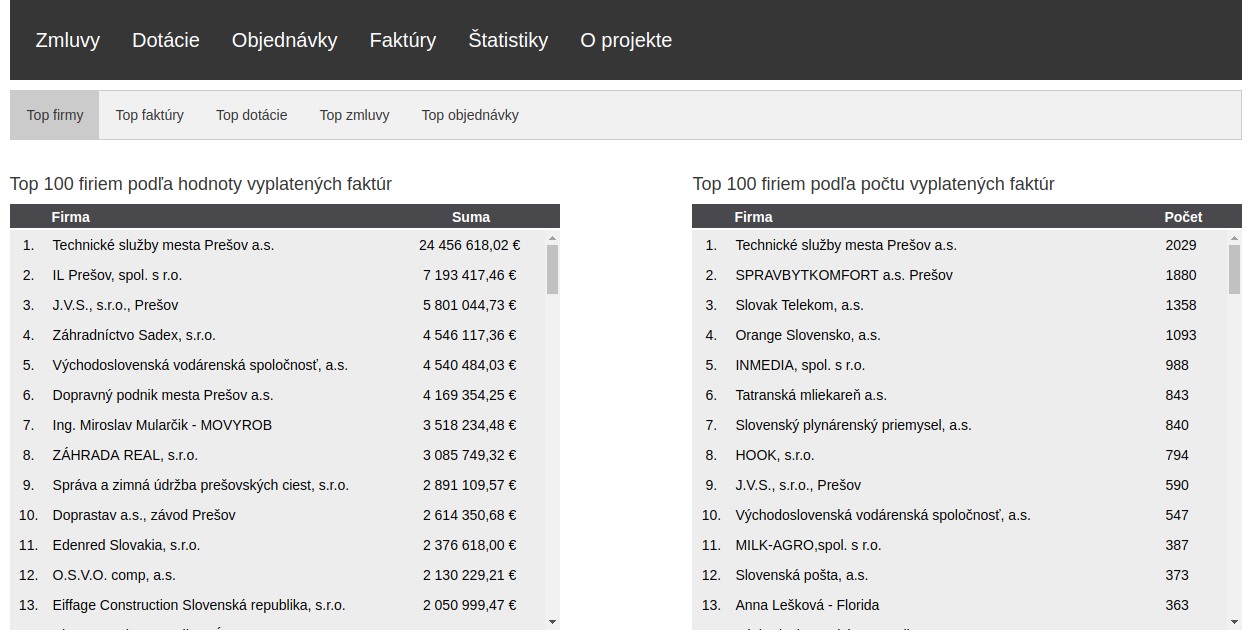
\includegraphics[scale=0.30]{pictures/statistics.png}
  \caption{Tab with the top companies by paid Prešov's invoices.}
    \label{fig:webapp-topcompanies}
  \end{center}
\end{figure}

\begin{figure}[H]
  \begin{center}
  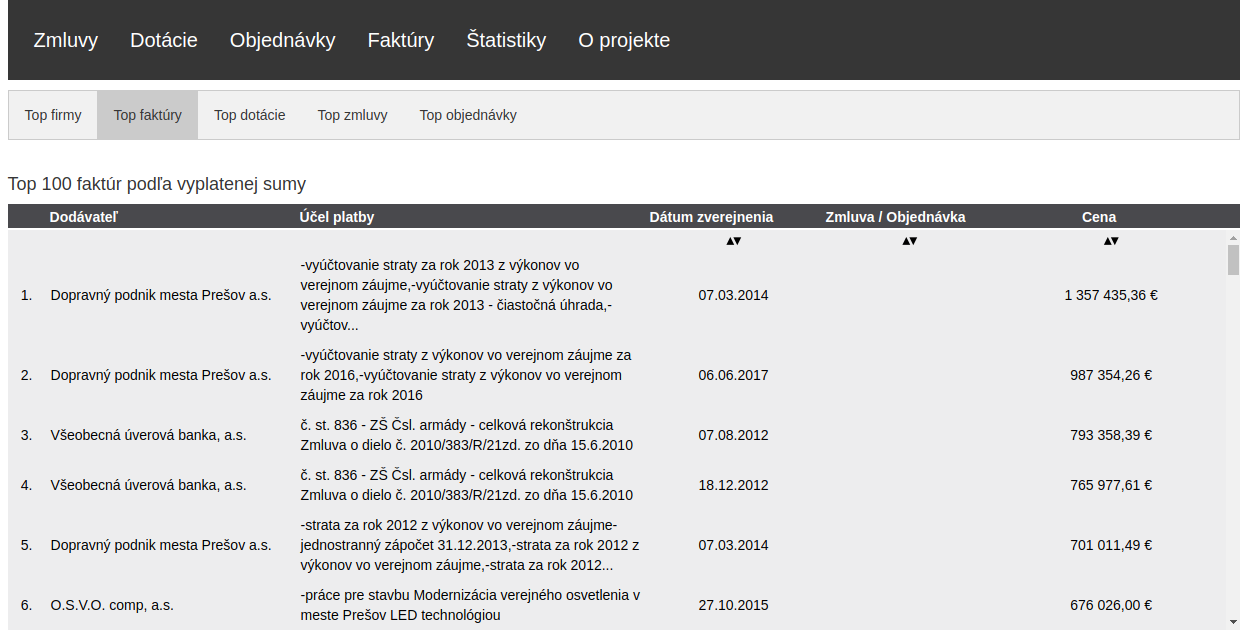
\includegraphics[scale=0.30]{pictures/topInvoices.png}
  \caption{Tab with the top invoices by paid amount.}
    \label{fig:webapp-topinvoices}
  \end{center}
\end{figure}

\begin{figure}[H]
  \begin{center}
  
\includegraphics[scale=0.35]{pictures/orderNotFound.png}
  \caption{Picture showing the way the web application handles record, that was not found.}
    \label{fig:webapp-contract-notfound}
  \end{center}
\end{figure}
\bibliographystyle{csn690}
\begin{thebibliography}{9}
\bibitem{opendatahandbook} 
\textit{What is Open Data? [online].}
[cit. 2018-02-28]. Available from: \url{http://opendatahandbook.org/guide/en/what-is-open-data/} 

\bibitem{opendefinition} 
Open Definition.
\textit{Open Definition 2.0 [online].}
[cit. 2018-03-02]. Available from: \url{http://opendefinition.org/od/2.0/en/} 

\bibitem{creativecommons}
\textit{Creative Commons licenses [online].}
[cit. 2018-19-04]. Available from: \url{https://creativecommons.org/licenses/}

\bibitem{europeandataportal} 
European Data Portal.
\textit{What is open data? [online].}
[cit. 2018-03-02]. Available from: \url{https://www.europeandataportal.eu/elearning/en/module1} 

\bibitem{opendatahandbookfileformats}
\textit{File formats [online].}
[cit. 2018-03-02]. Available from: \url{http://opendatahandbook.org/guide/en/appendices/file-formats/} 

\bibitem{5stardata}
\textit{5 star data [online].}
[cit. 2018-23-03]. Available from: \url{http://5stardata.info/en/} 

\bibitem{opendatabarometer}
\textit{Open data barometer [online].}
[cit. 2018-25-03]. Available from: \url{https://opendatabarometer.org/}

\bibitem{UKopendatagov}
\textit{Government Computing [online].}
[cit. 2018-25-03]. Available from: \url{http://central-government.governmentcomputing.com/features/who-is-leading-open-data-in-europe-walking-the-open-data-talk-5653451}

\bibitem{lmiforall}
\textit{LMI for all [online].}
[cit. 2018-25-03]. Available from: \url{http://www.lmiforall.org.uk/about-lmi-for-all/}

\bibitem{EUopendataportal}
\textit{European Union Open Data Portal [online].}
[cit. 2018-13-04]. Available from: \url{http://data.europa.eu/euodp/en/home/}

\bibitem{eudataportal}
\textit{European Data Portal[online].}
[cit. 2018-25-03]. Available from: \url{https://www.europeandataportal.eu/en/what-we-do/our-activities}

\bibitem{eudataportalfactsheet}
\textit{European Data Portal Factsheet [online].}
[cit. 2018-26-03]. Available from: \url{https://www.europeandataportal.eu/sites/default/files/country-factsheet_slovakia_2017.pdf}

\bibitem{slovakactionplan}
\textit{Action plan of Slovak Open data 2017-2019 [online].}
[cit. 2018-26-03]. Available from: \url{http://www.rokovania.sk/Rokovanie.aspx/BodRokovaniaDetail?idMaterial=26262}

\bibitem{crz}
\textit{Central Registry of Contracts [online].}
[cit. 2018-30-03]. Available from: \url{http://www.vlada.gov.sk/od-1-januara-2011-zacal-fungovat-centralny-register-zmluv/}

\bibitem{joinupcrz}
\textit{Joinup - Slovakian online central register contracts - crs [online].}
[cit. 2018-30-03]. Available from: \url{https://joinup.ec.europa.eu/document/slovakian-online-central-register-contracts-crs}

\bibitem{otvorenezmluvy}
\textit{Otvorené zmluvy [online].}
[cit. 2018-04-04]. Available from: \url{http://www.otvorenezmluvy.sk/o-projekte}

\bibitem{opengovernmentpartnership}
\textit{Open Government Partnership [online].}
[cit. 2018-06-04]. Available from: \url{https://www.opengovpartnership.org/about/about-ogp}

\bibitem{itapa}
\textit{ITAPA events [online].}
[cit. 2018-19-04]. Available from: \url{http://www.itapa.sk/o-itapa-podujatiach/}

\bibitem{nace}
\textit{What is a NACE Code? [online].}
[cit. 2018-11-05]. Available from: \url{https://siccode.com/en/pages/what-is-a-nace-code}

\end{thebibliography}

\chapter{Acronyms}
% \printglossaries
\begin{description}
	\item[IT] Information Technology
	\item[XML] Extensible markup language
	\item[JSON] JavaScript Object Notation
	\item[RDF] Resource Description Framework
	\item[CSV] Comma Separated Values
	\item[PDF] Portable Document Format
	\item[LMI] Labour market information
	\item[URL] Uniform Resource Locator
	\item[Java EE] Java Platform, Enterprise Edition
	\item[JSP] JavaServer Pages
	\item[HTTP] Hypertext Transfer Protocol
	\item[UI] User Interface
	\item[EFTA] European Free Trade Association 
\end{description}

% % % % % % % % % % % % % % % % % % % % % % % % % % % % 
% % Tuto kapitolu z výsledné práce ODSTRAŇTE.
% % % % % % % % % % % % % % % % % % % % % % % % % % % % 
% 
% \chapter{Návod k~použití této šablony}
% 
% Tento dokument slouží jako základ pro napsání závěrečné práce na Fakultě informačních technologií ČVUT v~Praze.
% 
% \section{Výběr základu}
% 
% Vyberte si šablonu podle druhu práce (bakalářská, diplomová), jazyka (čeština, angličtina) a kódování (ASCII, \mbox{UTF-8}, \mbox{ISO-8859-2} neboli latin2 a nebo \mbox{Windows-1250}). 
% 
% V~české variantě naleznete šablony v~souborech pojmenovaných ve formátu práce\_kódování.tex. Typ může být:
% \begin{description}
% 	\item[BP] bakalářská práce,
% 	\item[DP] diplomová (magisterská) práce.
% \end{description}
% Kódování, ve kterém chcete psát, může být:
% \begin{description}
% 	\item[UTF-8] kódování Unicode,
% 	\item[ISO-8859-2] latin2,
% 	\item[Windows-1250] znaková sada 1250 Windows.
% \end{description}
% V~případě nejistoty ohledně kódování doporučujeme následující postup:
% \begin{enumerate}
% 	\item Otevřete šablony pro kódování UTF-8 v~editoru prostého textu, který chcete pro psaní práce použít -- pokud můžete texty s~diakritikou normálně přečíst, použijte tuto šablonu.
% 	\item V~opačném případě postupujte dále podle toho, jaký operační systém používáte:
% 	\begin{itemize}
% 		\item v~případě Windows použijte šablonu pro kódování \mbox{Windows-1250},
% 		\item jinak zkuste použít šablonu pro kódování \mbox{ISO-8859-2}.
% 	\end{itemize}
% \end{enumerate}
% 
% 
% V~anglické variantě jsou šablony pojmenované podle typu práce, možnosti jsou:
% \begin{description}
% 	\item[bachelors] bakalářská práce,
% 	\item[masters] diplomová (magisterská) práce.
% \end{description}
% 
% \section{Použití šablony}
% 
% Šablona je určena pro zpracování systémem \LaTeXe{}. Text je možné psát v~textovém editoru jako prostý text, lze však také využít specializovaný editor pro \LaTeX{}, např. Kile.
% 
% Pro získání tisknutelného výstupu z~takto vytvořeného souboru použijte příkaz \verb|pdflatex|, kterému předáte cestu k~souboru jako parametr. Vhodný editor pro \LaTeX{} toto udělá za Vás. \verb|pdfcslatex| ani \verb|cslatex| \emph{nebudou} s~těmito šablonami fungovat.
% 
% Více informací o~použití systému \LaTeX{} najdete např. v~\cite{wikilatex}.
% 
% \subsection{Typografie}
% 
% Při psaní dodržujte typografické konvence zvoleného jazyka. České \uv{uvozovky} zapisujte použitím příkazu \verb|\uv|, kterému v~parametru předáte text, jenž má být v~uvozovkách. Anglické otevírací uvozovky se v~\LaTeX{}u zadávají jako dva zpětné apostrofy, uzavírací uvozovky jako dva apostrofy. Často chybně uváděný symbol "{} (palce) nemá s~uvozovkami nic společného.
% 
% Dále je třeba zabránit zalomení řádky mezi některými slovy, v~češtině např. za jednopísmennými předložkami a spojkami (vyjma \uv{a}). To docílíte vložením pružné nezalomitelné mezery -- znakem \texttt{\textasciitilde}. V~tomto případě to není třeba dělat ručně, lze použít program \verb|vlna|.
% 
% Více o~typografii viz \cite{kobltypo}.
% 
% \subsection{Obrázky}
% 
% Pro umožnění vkládání obrázků je vhodné použít balíček \verb|graphicx|, samotné vložení se provede příkazem \verb|\includegraphics|. Takto je možné vkládat obrázky ve formátu PDF, PNG a JPEG jestliže používáte pdf\LaTeX{} nebo ve formátu EPS jestliže používáte \LaTeX{}. Doporučujeme preferovat vektorové obrázky před rastrovými (vyjma fotografií).
% 
% \subsubsection{Získání vhodného formátu}
% 
% Pro získání vektorových formátů PDF nebo EPS z~jiných lze použít některý z~vektorových grafických editorů. Pro převod rastrového obrázku na vektorový lze použít rasterizaci, kterou mnohé editory zvládají (např. Inkscape). Pro konverze lze použít též nástroje pro dávkové zpracování běžně dodávané s~\LaTeX{}em, např. \verb|epstopdf|.
% 
% \subsubsection{Plovoucí prostředí}
% 
% Příkazem \verb|\includegraphics| lze obrázky vkládat přímo, doporučujeme však použít plovoucí prostředí, konkrétně \verb|figure|. Například obrázek \ref{fig:float} byl vložen tímto způsobem. Vůbec přitom nevadí, když je obrázek umístěn jinde, než bylo původně zamýšleno -- je tomu tak hlavně kvůli dodržení typografických konvencí. Namísto vynucování konkrétní pozice obrázku doporučujeme používat odkazování z~textu (dvojice příkazů \verb|\label| a \verb|\ref|).
% 
% \begin{figure}\centering
% 	
\includegraphics[width=0.5\textwidth, angle=30]{cvut-logo-bw}
% 	\caption[Příklad obrázku]{Ukázkový obrázek v~plovoucím prostředí}\label{fig:float}
% \end{figure}
% 
% \subsubsection{Verze obrázků}
% 
% % Gnuplot BW i barevně
% Může se hodit mít více verzí stejného obrázku, např. pro barevný či černobílý tisk a nebo pro prezentaci. S~pomocí některých nástrojů na generování grafiky je to snadné.
% 
% Máte-li například graf vytvořený v programu Gnuplot, můžete jeho černobílou variantu (viz obr. \ref{fig:gnuplot-bw}) vytvořit parametrem \verb|monochrome dashed| příkazu \verb|set term|. Barevnou variantu (viz obr. \ref{fig:gnuplot-col}) vhodnou na prezentace lze vytvořit parametrem \verb|colour solid|.
% 
% \begin{figure}\centering
% 	\includegraphics{gnuplot-bw}
% 	\caption{Černobílá varianta obrázku generovaného programem Gnuplot}\label{fig:gnuplot-bw}
% \end{figure}
% 
% \begin{figure}\centering
% 	\includegraphics{gnuplot-col}
% 	\caption{Barevná varianta obrázku generovaného programem Gnuplot}\label{fig:gnuplot-col}
% \end{figure}
% 
% 
% \subsection{Tabulky}
% 
% Tabulky lze zadávat různě, např. v~prostředí \verb|tabular|, avšak pro jejich vkládání platí to samé, co pro obrázky -- použijte plovoucí prostředí, v~tomto případě \verb|table|. Například tabulka \ref{tab:matematika} byla vložena tímto způsobem.
% 
% \begin{table}\centering
% 	\caption[Příklad tabulky]{Zadávání matematiky}\label{tab:matematika}
% 	\begin{tabular}{|l|l|c|c|}\hline
% 		Typ		& Prostředí		& \LaTeX{}ovská zkratka	& \TeX{}ovská zkratka	\tabularnewline \hline \hline
% 		Text		& \verb|math|		& \verb|\(...\)|	& \verb|$...$|		\tabularnewline \hline
% 		Displayed	& \verb|displaymath|	& \verb|\[...\]|	& \verb|$$...$$|	\tabularnewline \hline
% 	\end{tabular}
% \end{table}
% 
% % % % % % % % % % % % % % % % % % % % % % % % % % % % 

\chapter{Obsah přiloženého CD}

%upravte podle skutecnosti

\begin{figure}
	\dirtree{%
		.1 readme.txt\DTcomment{stručný popis obsahu CD}.
		.1 exe\DTcomment{adresář se spustitelnou formou implementace}.
		.1 src.
		.2 impl\DTcomment{zdrojové kódy implementace}.
		.2 thesis\DTcomment{zdrojová forma práce ve formátu \LaTeX{}}.
		.1 text\DTcomment{text práce}.
		.2 thesis.pdf\DTcomment{text práce ve formátu PDF}.
		.2 thesis.ps\DTcomment{text práce ve formátu PS}.
	}
\end{figure}

\end{document}
